\documentclass[12pt]{article}

\usepackage[utf8]{inputenc}
\usepackage[T2A]{fontenc}
\usepackage[english,russian]{babel}
\usepackage{amssymb}
\usepackage{graphicx}
\graphicspath{ {images/} }

\textwidth=431pt
\textheight=600pt
\hoffset=-30pt
\voffset=-30pt

\usepackage{graphicx}
\usepackage{amsmath}
\makeatletter
\renewcommand{\@oddhead}{%
\vbox{%
\hbox to \textwidth{\strut \textit{Statistical Analysis, Problem set 1, Usvyatsov Mikhail} \hfill }
%\hbox to\textwidth{Лист\hfill Страница~\arabic{page}~из 2}
\hrule
\vspace{12pt}
}}
\renewcommand{\@oddfoot}{}
\makeatother


\begin{document}

%\tableofcontents

%\newpage

\begin{center}
\textbf{Problem set 1 \\
Smoking and Lung Cancer \\
DUE: Wed. August 26, 2014 \\}
\end{center}

\begin{center}
	\begin{tabular}{|c|c|c|c|}
			\hline
			Observation No. & Country & \vtop{\hbox{\strut Cigarettes consumed}\hbox{\strut per capita in 1930 (X)}} & \vtop{\hbox{\strut Lung cancer deaths}\hbox{\strut per million people in 1950 (Y)}}\\
			\hline
			1 & Switzerland & 530 & 250 \\ 
			\hline
			2 & Finland & 1115 & 350 \\
			\hline
			3 & Great Britain & 1145 & 465 \\
			\hline
			4 & Canada & 510 & 150  \\
			\hline
			5 & Denmark & 380 & 165 \\
			\hline
	\end{tabular}
\end{center}
\newcounter{qcounter}
\section{Question 1}
\begin{list}{\alph{qcounter})~}{\usecounter{qcounter}}
\item The sample means of $X$ and $Y$, $\overline{X}$ and $\overline{Y}$.
\begin{gather*}
\overline{X} = \dfrac{\sum\limits_{n=1}^{n}{X_i}}{n} = 736\\
\overline{Y} = \dfrac{\sum\limits_{n=1}^{n}{Y_i}}{n} = 276
\end{gather*}
\item  The standard deviations of $X$ and $Y$, $s_X$ and $s_Y$.
\begin{gather*}
s_X = \sqrt{\dfrac{\sum\limits_{n=1}^{n}{\left(X_i - \overline{X}\right)^2}}{n-1}} = 364.4071\\
s_Y = \sqrt{\dfrac{\sum\limits_{n=1}^{n}{\left(Y_i - \overline{Y}\right)^2}}{n-1}} = 132.3537\\
\end{gather*}
\item The correlation coefficient, $r$, between $X$ and $Y$.
\begin{gather*}
r = Cov(X, Y) = \dfrac{\sum\limits_{n=1}^{n}{(X-\overline{X})(Y-\overline{Y})}}{s_Xs_Y(n-1)} =  0.9262529
\end{gather*}
\item $\hat{\beta_1}$, the OLS estimated slope coefficient from the regression $Y_i = \beta_0 + \beta_1X_i + u_i$.
\begin{gather*}
\hat{\beta_1} = \dfrac{\sum\limits_{n=1}^{n}{\left(X_i - \overline{X}\right)\left(Y_i - \overline{Y}\right)}}{\sum\limits_{n=1}^{n}{\left(X_i - \overline{X}\right)^2}} = 0.3364177
\end{gather*}
\item $\hat{\beta_1}$, the OLS estimated intercept term from the same regression.
\begin{gather*}
\beta_0 = \overline{Y} - \beta_1\overline{X} = 28.39656
\end{gather*}
\item $\hat{Y_i}$ , $i = 1,…,n$, the predicted values for each country from the regression.
\begin{gather*}
Y_i = \beta_0 + \beta_1X_i
\end{gather*}
\begin{center}
	\begin{tabular}{|c|c|c|c|c|c|}
		$\hat{Y_i}$ & 207 & 404 & 414 & 200 & 156\\
	\end{tabular}
\end{center}
\item  $\mu_i$, the OLS residual for each country. 
\begin{gather*}
\mu_i = Y_i - \hat{Y_i}
\end{gather*}
\begin{center}
	\begin{tabular}{|c|c|c|c|c|c|}
		\hline
		$\mu_i$ & 43.3 & -53.5 & 51.41 & -49.97 & 8.76\\
		\hline
	\end{tabular}
\end{center}
\end{list}

\section{Question 2}
Now calculate the statistics in question 1 using STATA. On the STATA output file, find and label the items in Question 1. \\
At this section I have used R. You can see code at the attached file.
The script output is:

[1] $\overline{X}$ = 736, $\overline{Y}$ = 276

[2] $s_x$ = 364.4071, $s_y$ = 132.3537

[3] r = 0.9263

[4] $\hat{\beta_1}$ and $\hat{\beta_0}$

Call: $lm(Y \sim X)$

Coefficients:

\begin{tabular}{cc}
	Intercept & data$X$\\
	28.3966 &  0.3364  
\end{tabular}

[5] $\hat{Y_i}$

Call: $predict(lm(Y \sim X))$

\begin{center}
	\begin{tabular}{|c|c|c|c|c|c|}
		206.6979 & 403.5023 & 413.5948 & 199.9696 & 156.2353\\
	\end{tabular}
\end{center}

\section{Question 3}
On graph paper or using a spreadsheet, graph the scatterplot of the five data points and the regression line. Be sure to label the axes, the data points, the residuals, and the slope and intercept of the regression line. (If you know the graphing commands in STATA you may do this using STATA. STATA has good graphing features but the commands are a little complicated and there is no need to learn them now – they will be covered later in the course.)

\begin{center}
  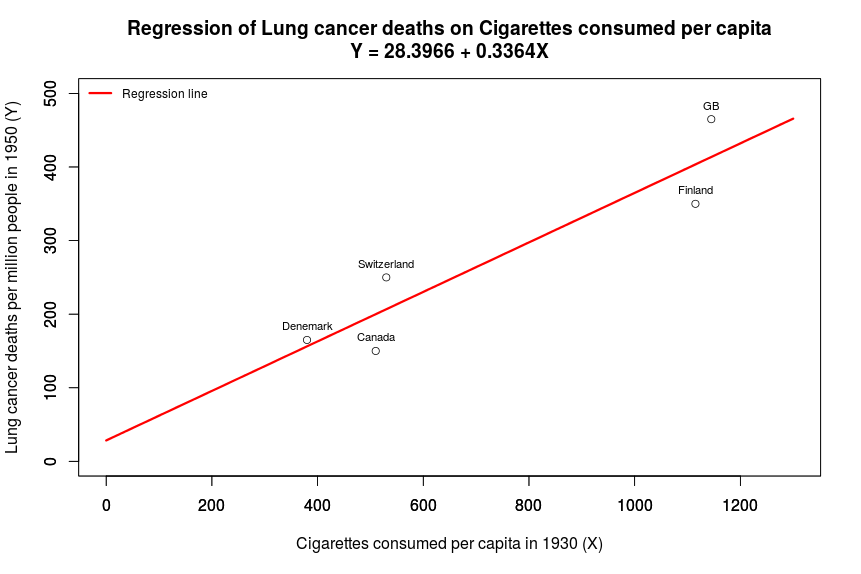
\includegraphics[width=15cm]{graph1}
\end{center}

\end{document}